\RequirePackage[]{optional}
%\RequirePackage[notslides]{optional}

\opt{slides}{
% Following for presentation mode
\documentclass[10pt]{beamer}
\usepackage{xmpmulti}
%usetheme{Berlin}
}
\opt{notslides}{
% Following for notes mode
\documentclass{article}
\usepackage{beamerarticle}
\usepackage{a4wide}
\usepackage{graphicx}
}

% Following for all modes
%\usepackage{auto-pst-pdf}
%\usepackage{pst-pdf}

\parindent=0ex
\parskip=1ex
\newcommand{\conv}{\ast}
\reversemarginpar

\title{Fourier series: Additional notes}
\author{}
\date{}

\begin{document}
\mode*  % no text out of frames
%\mode<article>{\setbeamertemplate{frametitle}{}}  % no frametitles

\begin{frame}
\titlepage
\end{frame}

\mode<article>{{\bf \LARGE Fourier series: Additional notes}}

\title{Fourier series: Additional notes}
\author{}
\date{}

\section{Linking Fourier series representations for signals}
\begin{frame}
  \frametitle<presentation>{Linking Fourier series representations for signals}
\end{frame}

\begin{frame}
\subsection{Rectangular waveform}
\frametitle<presentation>{Rectangular waveform}

Require FS expansion of signal $y(t)$ below:
\begin{center}
  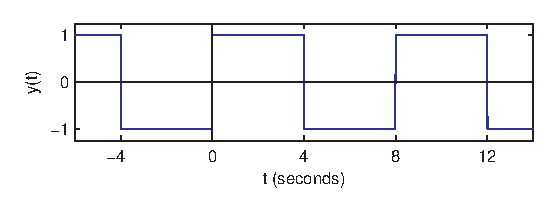
\includegraphics{fs_add_fig02}
\end{center}
Period $T=8$, so $\omega_0 = 2\pi/T = 2\pi/8 = \pi/4$ and the signal has a FS 
representation 
\begin{equation*}
  y(t) = \sum_{k=-\infty}^\infty d_k e^{j k (\pi/4) t}.
\end{equation*}
We could find the FS coefficients using the formula
\begin{equation*}
	d_k = \frac{1}{8} \int_0^8 y(t) e^{-j k (\pi/4) t} dt 
	= \frac{1}{8} \int_0^4 (1) e^{-j k (\pi/4) t} dt + \frac{1}{8} \int_4^8 (-1) e^{-j k (\pi/4) t} dt
\end{equation*}
but will do something simpler (and more interesting) instead.
\end{frame}

\begin{frame}
\frametitle{Rectangular waveform: derivative signal}

Consider instead the derivative of the previous signal $z(t) = \frac{d}{dt} y(t)$:
\begin{center}
  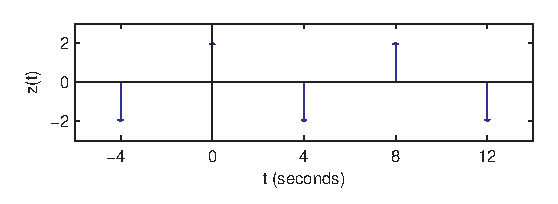
\includegraphics{fs_add_fig03}
\end{center}
This also has a period $T=8$, and a FS representation 
\begin{equation*}
  z(t) = \sum_{k=-\infty}^\infty f_k e^{j k (\pi/4) t}.
\end{equation*}
Note that this is of the same form as the FS for $y(t)$, just
with a different set of coefficients.
\end{frame}

\begin{frame}
\frametitle{FS coefficients for derivative signal}

Find the FS coefficients for $z(t)$ by integrating over one 
complete period.  Choose the interval $t=-2$ to $t=6$ to avoid
integrating over half a Dirac delta (we're free to choose the 
integration range as long as we integrate over one period):
\begin{align*}
  f_k &= \frac{1}{8} \int_{-2}^6 z(t) e^{-j k (\pi/4) t} dt
  = \frac{1}{8} \int_{-2}^6 [2 \delta(t) 
  - 2 \delta(t-4)] e^{-j k (\pi/4) t} dt \\
  &= \frac{2}{8} \int_{-2}^6 \delta(t) e^{-j k (\pi/4) t} dt 
  - \frac{2}{8} \int_{-2}^6 \delta(t-4) e^{-j k (\pi/4) t} dt \\
  &= \frac{1}{4} \int_{-2}^6 \delta(t) e^{-j k (\pi/4) 0} dt 
  - \frac{1}{4} \int_{-2}^6 \delta(t-4) e^{-j k (\pi/4) 4} dt \\
  &= \frac{1}{4} e^{-j k (\pi/4) 0} \int_{-2}^6 \delta(t) dt 
  - \frac{1}{4} e^{-j k (\pi/4) 4} \int_{-2}^6 \delta(t-4)  dt \\
  &= \frac{1}{4} e^{-j k (\pi/4) 0} - \frac{1}{4} e^{-j k (\pi/4) 4} \\
  &= \frac{1}{4} (1 - e^{-j k \pi}).
\end{align*}
\end{frame}

\begin{frame}
\frametitle{Rectangular waveform:  Relationship between coefficients}

Since $z(t) = \frac{d}{dt} y(t)$, we can find a relationship between
the coefficients:
\begin{align*}
  z(t) &= \frac{d}{dt} y(t) = \frac{d}{dt} \left[
  \sum_{k=-\infty}^\infty d_k e^{j k (\pi/4) t} \right] 
  = \sum_{k=-\infty}^\infty \frac{d}{dt} \left[
  d_k e^{j k (\pi/4) t} \right] \\
  &= \sum_{k=-\infty}^\infty d_k \frac{d}{dt} \left[
  e^{j k (\pi/4) t} \right]
  = \sum_{k=-\infty}^\infty d_k j k (\pi/4) e^{j k (\pi/4) t}.
\end{align*}
But the FS for $y(t)$ is of the same form
\begin{equation*}
  z(t) = \sum_{k=-\infty}^\infty f_k e^{j k (\pi/4) t},
\end{equation*}
so each of the coefficients must be equal:
\begin{equation*}
  f_k = d_k j k (\pi/4) = j k \frac{\pi}{4} d_k.
\end{equation*}
\end{frame}

\begin{frame}
\frametitle<presentation>{Rectangular waveform:  Relationship between coefficients}
The FS coefficients $d_k$ (for the square wave) are related to the
coefficients $f_k$ (for the derivative signal) by
\begin{equation*}
  d_k = \frac{1}{j k \pi/4} f_k.
\end{equation*}
This formula will work for all $k$ except $k=0$ (where it becomes an indeterminate 
form --- division by zero).  
To find $d_0$, just go back to $y(t)$ and calculate directly:
\begin{equation*}
  d_0 = \int_0^8 y(t) dt = 
  \frac{1}{8} \int_0^4 (1) dt + \frac{1}{8} \int_4^8 (-1) dt = 0.
\end{equation*}
Therefore the FS coefficients $d_k$ of $y(t)$ are
\begin{equation*}
  d_k = \begin{cases}
  0 \qquad & (k=0) \\
  \frac{1}{j k \pi} (1 - e^{-j k \pi}) \qquad & (k \neq 0).
  \end{cases}
\end{equation*}
\end{frame}

\begin{frame}
\frametitle{Rectangular wave:  FS coefficient plot}

\begin{center}
  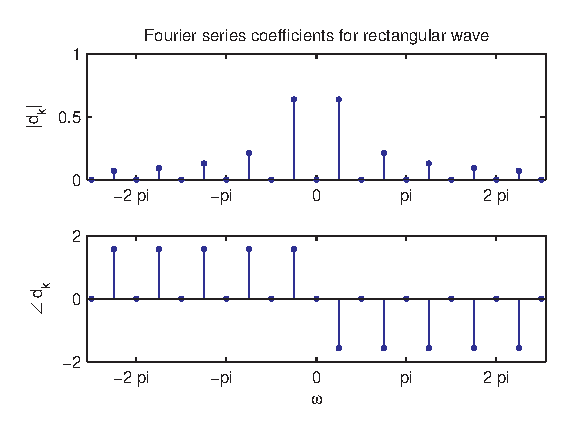
\includegraphics{fs_add_fig05}
\end{center}
\end{frame}

\begin{frame}
\subsection{Triangular waveform}
\frametitle<presentation>{Triangular waveform}

Now find the FS coefficients of $x(t)$ below:
\begin{center}
  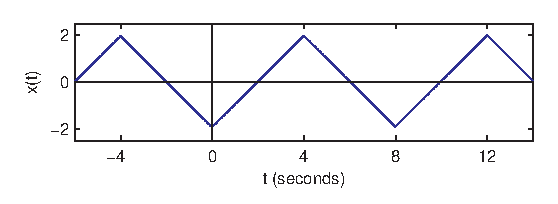
\includegraphics{fs_add_fig01}
\end{center}
Period $T=8$, so $\omega_0 = 2\pi/T = 2\pi/8 = \pi/4$ and the signal has a FS 
representation 
\begin{equation*}
  x(t) = \sum_{k=-\infty}^\infty c_k e^{j k (\pi/4) t}.
\end{equation*}
\end{frame}

\begin{frame}
\frametitle{Triangular waveform:  FS coefficients}

We could find the FS coefficients using the formula
\begin{align*}
	c_k &= \frac{1}{8} \int_0^8 x(t) e^{-j k (\pi/4) t} dt \\
	&= \frac{1}{8} \int_0^4 x(t) e^{-j k (\pi/4) t} dt
	+ \frac{1}{8} \int_4^8 x(t) e^{-j k (\pi/4) t} dt \\
	&= \frac{1}{8} \int_0^4 (t-2) e^{-j k (\pi/4) t} dt
	+ \frac{1}{8} \int_4^8 (4-t) e^{-j k (\pi/4) t} dt
\end{align*}
so
\mode<presentation>{
\begin{multline*}
	c_k = \frac{1}{8} \int_0^4 t e^{-j k (\pi/4) t} 
	- \frac{2}{8} \int_0^4 e^{-j k (\pi/4) t} \\
	+ \frac{4}{8} \int_4^8 e^{-j k (\pi/4) t} 
	- \frac{1}{8} \int_4^8 t e^{-j k (\pi/4) t}.
\end{multline*}
}
\mode<article>{
\begin{equation*}
	c_k = \frac{1}{8} \int_0^4 t e^{-j k (\pi/4) t} 
	- \frac{2}{8} \int_0^4 e^{-j k (\pi/4) t} 
	+ \frac{4}{8} \int_4^8 e^{-j k (\pi/4) t} 
	- \frac{1}{8} \int_4^8 t e^{-j k (\pi/4) t}.
\end{equation*}
}
Two of these integrals are easy, but two have to be done by parts.

\mode<presentation>{{\bf Exercise 1:} Calculate the FS coefficients for the above.} 
\mode<article>{Calculate the FS coefficients for the above.\marginpar{\bf Exercise 1:}}
\end{frame}

\begin{frame}
\frametitle{Triangular waveform:  alternative method}
Consider instead the signal $y(t) = \frac{d}{dt} x(t)$:
\begin{center}
  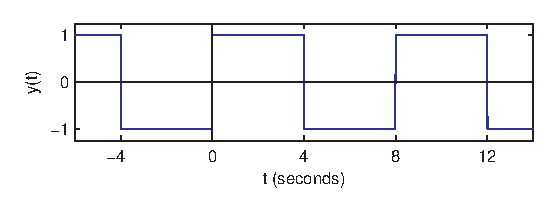
\includegraphics{fs_add_fig02}
\end{center}
This also has a period $T=8$, and a FS representation 
\begin{equation*}
  y(t) = \sum_{k=-\infty}^\infty d_k e^{j k (\pi/4) t}
\end{equation*}
and the coefficients were found earlier to be
\begin{equation*}
  d_k = \begin{cases}
  0 \qquad & (k=0) \\
  \frac{1}{j k \pi} (1 - e^{-j k \pi}) \qquad & (k \neq 0).
  \end{cases}
\end{equation*}
\end{frame}

\begin{frame}
\frametitle{Triangular waveform:  Relationship between coefficients}

As before, since $y(t) = \frac{d}{dt} x(t)$ a relationship exists between
the coefficients:
\begin{align*}
  y(t) &= \frac{d}{dt} x(t) = \frac{d}{dt} \left[
  \sum_{k=-\infty}^\infty c_k e^{j k (\pi/4) t} \right] 
  = \sum_{k=-\infty}^\infty \frac{d}{dt} \left[
  c_k e^{j k (\pi/4) t} \right] \\
  &= \sum_{k=-\infty}^\infty c_k \frac{d}{dt} \left[
  e^{j k (\pi/4) t} \right]
  = \sum_{k=-\infty}^\infty c_k j k (\pi/4) e^{j k (\pi/4) t}.
\end{align*}
But the FS for $y(t)$ is of the same form
\begin{equation*}
  y(t) = \sum_{k=-\infty}^\infty d_k e^{j k (\pi/4) t},
\end{equation*}
so each of the coefficients must be equal:
\begin{equation*}
  d_k = c_k j k (\pi/4) = j k \frac{\pi}{4} c_k.
\end{equation*}
\end{frame}

\begin{frame}
\frametitle<presentation>{Triangular waveform:  Relationship between coefficients}
The FS coefficients $c_k$ (for the triangular wave) can therefore be 
found from the coefficients $d_k$ (for the square wave) using
\begin{equation*}
  c_k = \frac{1}{j k \pi/4} d_k,
\end{equation*}
as long as $k \neq 0$.  To find $c_0$, just go
back to $x(t)$ and calculate directly:
\begin{equation*}
  c_0 = \frac{1}{8} \int_0^8 x(t) dt = 
  \frac{1}{8} \int_0^4 (t-2) dt + \frac{1}{8} \int_4^8 (4-t) dt = 0.
\end{equation*}
The FS coefficients for $x(t)$ are therefore
\begin{equation*}
  c_k = \begin{cases}
  0 \qquad & (k=0) \\
  \frac{1}{j k \pi/4} \frac{1}{j k \pi} (1 - e^{-j k \pi}) \qquad & (k \neq 0).
  \end{cases}
\end{equation*}
No integration by parts needed!
\end{frame}

\begin{frame}
\frametitle{Triangular wave:  FS coefficient plot}

\begin{center}
  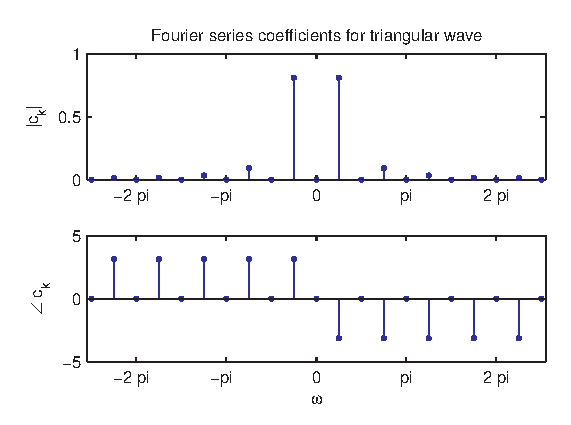
\includegraphics{fs_add_fig06}
\end{center}
\end{frame}

\begin{frame}[fragile,shrink=20]
\frametitle{Check with Matlab}
\begin{verbatim}
j = sqrt(-1);  % to be sure
tv = -6:0.001:14;  % time values (a row vector)
xv = zeros(size(tv));  % signal values initially zero
N = 10;  % highest term in synthesis equation
for k=-N:N
  % Current complex exponential values (a row vector)
  xcv = exp(j*k*pi/4*tv);
  
  % Coefficient for current complex exponential
  if k==0
    ck = 0;  % DC
  else
    ck = 4/((j*k*pi)^2)*(1 - exp(-j*k*pi));  % formula
    %ck = 1/(j*k*pi)*(1 - exp(-j*k*pi));  % y(t)
    %ck = 1/4*(1 - exp(-j*k*pi));  % z(t)
  end
  
  % Add scaled complex exponential to signal values
  xv = xv + ck*xcv;
end
plot(tv,real(xv));  % the values *should* be real
\end{verbatim}
\mode<presentation>{{\bf Exercise 2:} Run the above code in Matlab.}
\mode<article>{Run the above code in Matlab.\marginpar{\bf Exercise 2:}}
\end{frame}

Open Matlab, type {\tt edit fs\_reconstruct.m}, press enter.
Copy the code above into the editor, save it, and run the file.  You will see the 
reconstruction of the triangular wave using {\tt N} terms.  Try different values 
$N$.  Look at the code and find the line that calculates the formula, and try the
formulas for the two derivative signals.  What's going on for the impulse train
signal?

\begin{frame}
\frametitle{Triangular wave:  synthesis}
\begin{center}
  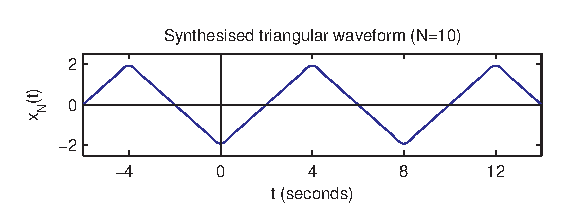
\includegraphics{fs_add_fig04}
\end{center}

\mode<presentation>{{\bf Exercise 3:} Find the FS of the signal below:}
\mode<article>{Find the FS of the signal below:\marginpar{\bf Exercise 3:}}
\begin{center}
  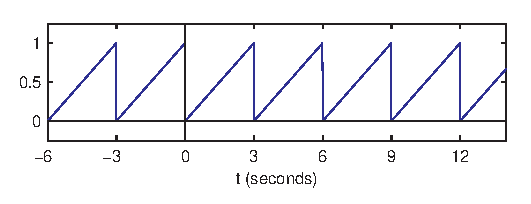
\includegraphics{fs_add_fig07}
\end{center}
\end{frame}

\begin{frame}
\frametitle{Notes}
Some interesting observations:
\begin{enumerate}
\item Triangular waveform is continuous (quite smooth), but has discontinuous derivatives --- 
  FS coefficients decreases as $\frac{1}{\omega^2}$ --- they decrease very quickly as
  frequency increases.
\item Rectangular waveform is discontinuous (less smooth than triangular waveform) --- 
  FS coefficients decreases as $\frac{1}{\omega}$ --- more slowly.
\item Smooth waveforms generally contain less high frequency components --- their coefficients
go to zero closer to the origin in the frequency domain.
\item Alternatively, to reconstruct a signal with fast variations (i.e. discontinuities)
  requires large components at high frequencies.
\end{enumerate}

\end{frame}

\begin{frame}
\frametitle{Linking coefficients for other transformations}
Consider a signal $x(t)$ with period $T$:  it has a FS expansion
\begin{equation*}
  x(t) = \sum_{k=-\infty}^\infty c_k e^{j k \omega_0 t}
\end{equation*}
with $\omega_0 = 2\pi/T$.

Let $y(t)$ be a signal related to $x(t)$.  If $y(t)$ is also
periodic with period $T$ then it has a FS expansion
\begin{equation*}
  y(t) = \sum_{k=-\infty}^\infty d_k e^{j k \omega_0 t}.
\end{equation*}
and the coefficients $c_k$ and $d_k$ are related.
\end{frame}

\begin{frame}
\frametitle{Relationship for shift transformation}
Consider the case where $y(t) = x(t-a)$ for some $a$.  Clearly
$y(t)$ is periodic with the same period as $x(t)$, and
\begin{align*}
  y(t) &= x(t-a) = \sum_{k=-\infty}^\infty c_k e^{j k \omega_0 (t-a)} 
  = \sum_{k=-\infty}^\infty c_k e^{j k \omega_0 t} e^{-j k \omega_0 a} \\
  &= \sum_{k=-\infty}^\infty (c_k e^{-j k \omega_0 a}) e^{j k \omega_0 t} 
  = \sum_{k=-\infty}^\infty d_k e^{j k \omega_0 t}.
\end{align*}
The coefficients are therefore related by
\begin{equation*}
  d_k = c_k e^{-j k \omega_0 a}
\end{equation*}
Thus a shift corresponds to a change in the phase of each coefficient, 
where the amount of the change is proportional to the size of the shift.
\end{frame}

\begin{frame}

\mode<presentation>{{\bf Exercise 4:} Find the FS of the signal below, using the series coefficients $c_k$ found earlier for $x(t)$:}
\mode<article>{Find the FS of the signal below, using the series coefficients $c_k$ found earlier for $x(t)$:\marginpar{\bf Exercise 4:}}
\begin{center}
  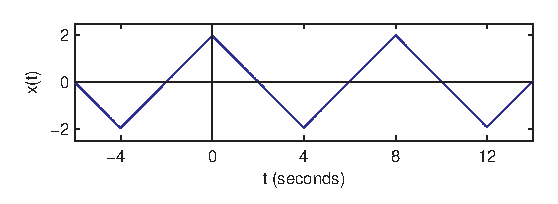
\includegraphics{fs_add_fig08}
\end{center}
\end{frame}

\end{document}
